\documentclass[border=10pt]{standalone}
\usepackage{tikz}
\usepackage[utf8]{inputenc}
\usepackage[T1]{fontenc}
\usetikzlibrary{patterns}
\usetikzlibrary{arrows.meta}
\usetikzlibrary{decorations.pathreplacing} % NECESSÁRIO para brace

\begin{document}

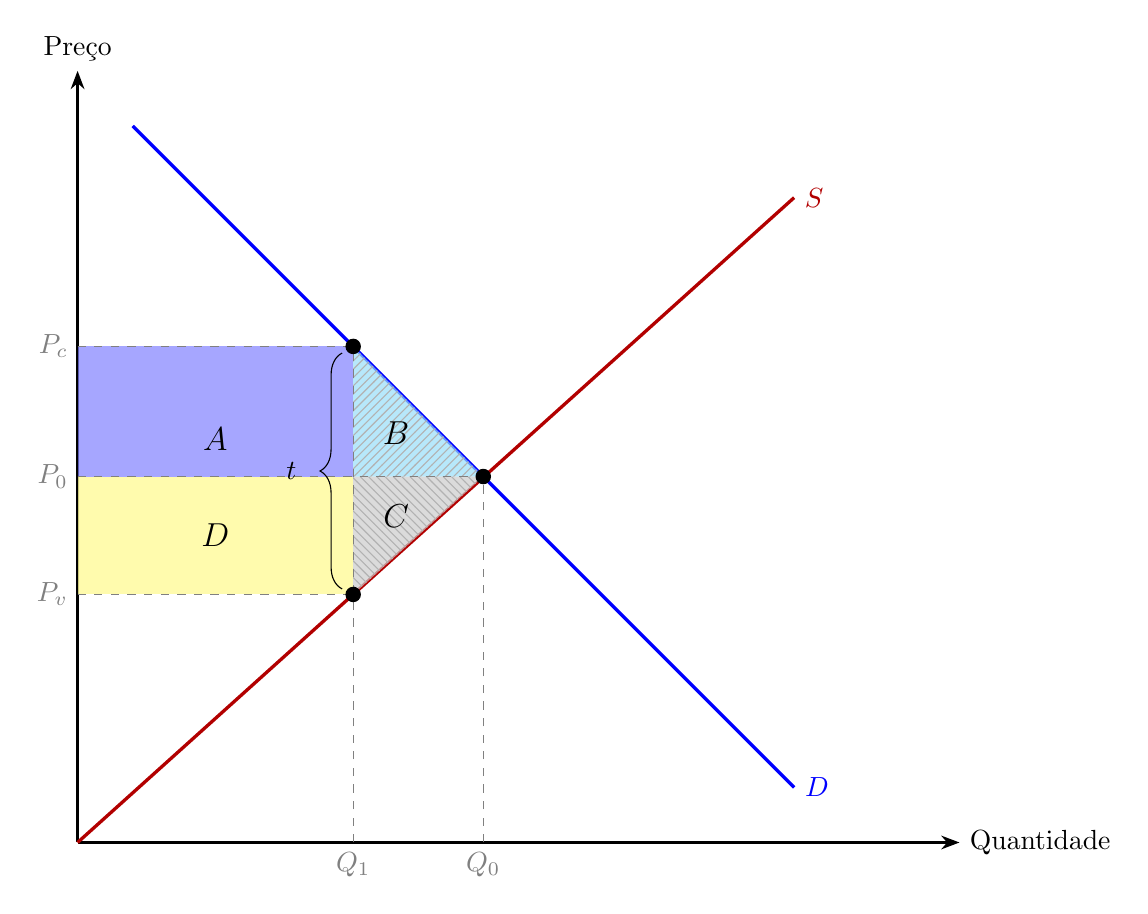
\begin{tikzpicture}[scale=1.4, >=Stealth]
    
    % Eixos
    \draw[thick,->] (0,0) -- (8,0) node[right] {Quantidade};
    \draw[thick,->] (0,0) -- (0,7) node[above] {Preço};
    
    % Curvas de oferta e demanda - mais verticais
    \draw[blue, very thick, domain=0.5:6.5] plot (\x, {7.0 - 1.0*\x}) node[right] {$D$};
    \draw[red!70!black, very thick, domain=0:6.5] plot (\x, {0.9*\x}) node[right] {$S$};
    
    % Coordenadas importantes
    % Novas curvas: D: y = 7.0 - 1.0*x, S: y = 0.9*x
    % Equilíbrio: 7.0 - 1.0*x = 0.9*x => 7.0 = 1.9*x => x = 3.68, y = 3.32
    \def\Qeq{3.68}      % Quantidade de equilíbrio sem imposto
    \def\Qt{2.5}        % Quantidade com imposto (reduzido para aumentar diferença)
    \def\Peq{3.32}      % Preço de equilíbrio sem imposto
    \def\Pb{4.5}        % Preço pago pelos compradores (com imposto) - mais elevado
    \def\Ps{2.25}       % Preço recebido pelos vendedores (menos imposto) - mais baixo
    
    % Área A (perda excedente do consumidor - azul)
    \fill[blue!50, opacity=0.7] (0,\Pb) rectangle (\Qt,\Peq);
    
    % Área D (receita do governo dos consumidores - amarelo claro)
    \fill[yellow!40, opacity=0.8] (0,\Peq) rectangle (\Qt,\Ps);
    
    % Área B (perda de peso morto do lado da demanda) - com textura cinza
    \fill[cyan!40, opacity=0.7] (\Qt,\Pb) -- (\Qt,\Peq) -- (\Qeq,\Peq) -- cycle;
    \fill[pattern=north east lines, pattern color=gray!60] (\Qt,\Pb) -- (\Qt,\Peq) -- (\Qeq,\Peq) -- cycle;
    
    % Área C (perda de peso morto do lado da oferta) - com textura
    \fill[gray!40, opacity=0.7] (\Qt,\Peq) -- (\Qt,\Ps) -- (\Qeq,\Peq) -- cycle;
    \fill[pattern=north west lines, pattern color=gray!60] (\Qt,\Peq) -- (\Qt,\Ps) -- (\Qeq,\Peq) -- cycle;
    
    % Linhas tracejadas horizontais
    \draw[dashed, gray] (0,\Pb) node[left] {$P_c$} -- (\Qt,\Pb);
    \draw[dashed, gray] (0,\Peq) node[left] {$P_0$} -- (\Qeq,\Peq);
    \draw[dashed, gray] (0,\Ps) node[left] {$P_v$} -- (\Qt,\Ps);
    
    % Linhas tracejadas verticais
    \draw[dashed, gray] (\Qt,0) node[below] {$Q_1$} -- (\Qt,\Pb);
    \draw[dashed, gray] (\Qeq,0) node[below] {$Q_0$} -- (\Qeq,\Peq);
    
    % Rótulos das áreas
    % Área A: retângulo (0, Peq) a (Qt, Pb)
    % Centro: ((0+Qt)/2, (Peq+Pb)/2) = (1.25, 3.66)
    \node at (1.25, 3.66) {\large $A$};
    % Área B: triângulo (Qt, Pb), (Qt, Peq), (Qeq, Peq)
    % Centróide: ((Qt+Qt+Qeq)/3, (Pb+Peq+Peq)/3) = ((2.5+2.5+3.68)/3, (4.5+3.32+3.32)/3) = (2.89, 3.71)
    \node at (2.89, 3.71) {\large $B$};
    % Área C: triângulo (Qt, Peq), (Qt, Ps), (Qeq, Peq)
    % Centróide: ((Qt+Qt+Qeq)/3, (Peq+Ps+Peq)/3) = ((2.5+2.5+3.68)/3, (3.32+2.25+3.32)/3) = (2.89, 2.96)
    \node at (2.89, 2.96) {\large $C$};
    % Área D: retângulo (0, Ps) a (Qt, Peq)
    % Centro: ((0+Qt)/2, (Ps+Peq)/2) = (1.25, 2.79)
    \node at (1.25, 2.79) {\large $D$};
    
    % Pontos de equilíbrio
    \fill (\Qeq,\Peq) circle (2pt);
    \fill (\Qt,\Pb) circle (2pt);
    \fill (\Qt,\Ps) circle (2pt);
    
    % Chave mostrando o imposto - do lado esquerdo de Q1
    % Usando delimitador LaTeX apropriado com fonte menor
    \draw[decorate,decoration={brace,amplitude=8pt}]
    (2.4,2.3) -- (2.4,4.44) node[midway,left=13pt] {$t$};
    % \node at (\Qt+0.3,{(\Ps+\Pb)/2}) [left, scale=2.9] {\tiny $\Biggl\{$};
    % \node at (\Qt-0.45,{(\Ps+\Pb)/2}) [left] {$t$};
    
\end{tikzpicture}

\end{document}
